\addbibresource{reference.bib}

\chapter{Atlas TPX}\label{atlas}
Atlas TPX, síť 16\footnote{V průběhu LS3\textsuperscript{\ref{ls}} (plánováno 2017 - 2018) je plánováno rozšíření teto sítě o nové detektory} hybridních částicových pixelových detektorů typu Timepix \ref{det:tim}, nainstalovaných na různé pozice experimentu Atlas na LHC\footnote{z angl. Large Hadron Collider} v CERN během LS2\footnote{\label{ls}z angl. long shutdown - dlouhodobá technologická přestávka LHC} (leden 2013 až březen 2015) je následníkem svého předchůdce - sítě Atlas MPX (viz \ref{atlas:mpx}). Hlavní motivací výměny této sítě bylo využití nových technologií, především pak nového detekčního čipu Timepix. Ten na rozdíl od svého předchůdce Medipix2 \ref{det:med} umožňuje rozšíření naměřené informace i o časovou oblast (viz \ref{det:tim}). To nově umožňuje provozovat detektory v módech TOA\footnote{z angl. Time of Arrival - čas příletu částice v hodinových cyklech detektoru od začátku akvizice} a TOT\footnote{z angl. Time Over Treshold - počet hodinových cyklů, kdy komparační napětí je větší, než referenční (ekvivalent energie deponované částice, viz kapitola \ref{calib})}. 

Další změnou oproti svému předchůdci je, že každý detektor obsahuje dva detekční čipy s tloušťkami $300~\mu m$ a $500~\mu m$, umístěné předními stranami k sobě - viz \ref{fig:tpx_detector_layers}. To přináší možnost měřit koincidence - když částice projde oběma vrstvami  detektoru a zároveň v každé nechá jisté měřitelné množství své energie, je detekována oběma vrstvami a je možné zpětně zrekonstruovat její trajektorii. Tyto koincidence se nejsnáze detekují, pokud oba Timepix čipy pracují v módu TOA - jelikož rychlost částic se blíží rychlosti světla, je vysoce pravděpodobné, že zasažené pixely budou mít stejnou hodnotu.


\begin{figure}[th]
	\begin{center}
		\begin{subfigure}{6cm}
			\includegraphics[width=6cm]{figures/tpx_lay.png}	
			\caption{Vrstvy detektoru}
			\label{fig:tpx_detector_layers}
		\end{subfigure}
		\hspace{0.5cm}
		\begin{subfigure}{5cm}
			\includegraphics[width=5cm]{figures/tpx_conv.png}
			\caption{Rozmístění konvetorů}
			\label{fig:tpx_detector_convertors}
		\end{subfigure}
		\caption{Atlas TPX detektor - vrstvy a rozmístění konvertorů}
		\label{fig:tpx_detector}
	\end{center}			
\end{figure}

Mezi vrstvami detektoru je umístěn konvertující materiál pro detekci termálních a rychlých neutronů. Rozmístění těchto konvertorů je na obrázku \ref{fig:tpx_detector_convertors}.

Hlavním úkolem Atlas TPX experimentu je online monitorování spektrálních charakteristik velice různorodého radiačního prostředí Atlas experimentu, založené na prostorovém uspořádání sítě a (vzhledem k aktuálním módu detektoru) i na informaci o deponované energii zainteragovaných částic, či na času jejich interakce. 


Detektory, instalované blízko interakčnímu bodu, jsou rovněž použity jako monitory integrované luminozity, což je veličina, která udává počet realizovaných srážek, resp. s intenzitou svazku urychlovače. Podle \cite{wagner:o_lhc} je to veličina, která v případě srážení dvou proti sobě letících svazků ukazuje, jaký je součin počtů částic v jednotlivých svazcích prolétajících jednotkovou plochou v srážkové oblasti, vynásobený počtem obletů svazků za jednotku času (nejčastěji se vyjadřuje v jednotkách na centimetr čtvereční a sekundu).

\begin{figure}[ht]
	\begin{center}
		\includegraphics[width=12cm]{figures/tpx_positions.png}
		\caption{Atlas TPX - přehledem rozmístění detektorů}
		\label{fig:tpx_positions}
	\end{center}
\end{figure}

%********************************************************************************
% Atlas MPX
%********************************************************************************
\section{Atlas MPX}\label{atlas:mpx}
Atlas MPX\cite{Vykydal200935}\cite{atlasmpx} je předchůdcem detektorové sítě Atlas TPX, který je v současné době plně nahrazen. Detektorová síť Atlas MPX se skládala z 16 Medipix2 detektorů, které byly instalovány na různé pozice Atlas detektoru. Hlavním cílem této sítě bylo měření vlastností radiačního pole uvnitř experimentu Atlas, jeho složení, spektroskopických charakteristik a částečně také přispěla k měření neutronů. 


Všechny detektory operovaly v tzv. \texttt{Medipix módu}, který se vyznačuje tím, že v rámci jedné akvizice počítá počet částic, které interagovaly pixelovou maticí detektoru a jejichž deponovaná energie byla vyšší, než prahová. Na obrázku \ref{fig:mpx_cluster} je znázorněn snímek z jednoho detektoru s detailem zachycených částic. Na obrázku vpravo nahoře je částice typu \texttt{heavy blob} (těžce nabitá částice, jejíž trajektorie byla kolmá s povrchem detektoru), vpravo dole je pak zachycena částice typu \texttt{heavy track} (také těžce nabitá částice, která ale přiletěla pod větším a proto zanechala větší stopu) - více klasifikaci částic se dočtete v podkapitole \ref{atlas:sw_arch}.


\begin{figure}[ht]
	\begin{center}
		\includegraphics[width=7cm]{figures/mpx_cluster.png}
		\caption{Snímek z Atlas MPX detektoru s výřezem zachycených částic (převzato z \cite{atlasmpx})}
		\label{fig:mpx_cluster}
	\end{center}
\end{figure}


Každý z těchto detektorů byl osazen $300~\mu m$ tlustým křemíkovým senzorem, který byl pokryt konvertory pro lepší detekční účinnost neutronů (obr. \ref{fig:mpx_lay}).

\begin{figure}[ht]
	\begin{center}
		\includegraphics[width=7cm]{figures/mpx-layers.jpg}
		\caption{Fotografie znázorňující Medipix2 detektor s neutronovými konvertory (převzato z \cite{Vykydal200935})}
		\label{fig:mpx_lay}
	\end{center}
\end{figure}

\subsection{Hardwarová a softwarová architektura sítě Atlas MPX}
Tato síť se skládala z 16 \texttt{Medipix2} \ref{det:med} detektorů, které byly pomocí USB vyčítacího rozhraní \texttt{FITPix} \ref{det:fitpix} připojeny ke třem počítačům (z důvodu distribuce toku dat a výkonu). Na každém počítači se o komunikaci s detektory staral software \texttt{Pixelman} \ref{det:pixelman}, který řídil akvizici dat, nastavování parametrů detektorů apod. 

Pro vzdálené obládání byl vyvinut plugin pro Pixelman, který umožňoval jeho rozšíření o TCP/IP ovládací vrstvu. Pomocí jednoduchého textového protokolu bylo tedy možné řídit každý ze třech uzlů. Pro tyto účely byla vyvinuta centrální řídící aplikace \cite{Turecek2011S45}, pomocí které bylo možné řídit řídit akvizici všech detektorů a nastavovat jejich parametry. Tato aplikace poskytovala webové rozhraní (obr. \ref{fig:mpx_web}), které díky tou dobou méně striktní CERNské politice síťové bezpečnosti bylo možné tento experiment ovládat odkudkoliv z internetu.

\begin{figure}[ht]
	\begin{center}
		\includegraphics[width=10cm]{figures/mpx_web.png}
		\caption{Atlas MPX - řídící aplikace (převzato z \cite{TurecekThesis2011})}
		\label{fig:mpx_web}
	\end{center}
\end{figure}

%********************************************************************************
% Hardwarová architektura
%********************************************************************************
\section{Hardwarová architektura}\label{atlas:hw_arch}
Při návrhu hardwarové architekty sítě Atlas TPX musela být zohledněna zvýšená intenzita radiačního a elektromagnetického pole v prostorách Atlas detektoru. Snahou proto bylo, co nejvíce hardwarových komponent umístit z dosahu tohoto pole. Z pohledu hardwarové instalace této detektorové sítě se prostory Atlas experimentu dělí na dvě části - \texttt{UX15} a \texttt{USA15} (viz obr. \ref{fig:tpx_hw_diagram}). V \texttt{UX15} se nachází vlastní experiment. V tomto prostoru byly umístěny jen detektory (na obr. \ref{fig:tpx_hw_diagram} \texttt{TPX01} až \texttt{TPX15}) a zbytek sítě byl instalován v \texttt{USA15}, kterou od zbytku experimentu dělí cca $60~m$ tlustá železobetonová stěna. Tady se nachází vyčítací elektronika a další nezbytný hardware.

\begin{figure}[t]
	\begin{center}
		\includegraphics[width=6cm]{figures/tpx_hw_diagram.png}
		\caption{Atlas TPX - diagram hw komponent}
		\label{fig:tpx_hw_diagram}
	\end{center}
\end{figure}

Na obrázku \ref{fig:tpx_hw_foto} je fotografie  těchto komponent. Jak již bylo zmíněno výše, detektor (z obr. \ref{fig:tpx_hw_foto}, na obr. \ref{fig:tpx_hw_diagram} jako \texttt{TPX01} až \texttt{TPX15}) se skládá z dvojice detekčních čipů \texttt{Timepix}, které jsou pomocí \texttt{LVDS} zesilovačů a cca $100~m$ dlouhých ethernetových kabelů propojeny se zařízením \texttt{AtlasPix} (obr. \ref{fig:tpx_hw_foto} dole), které vzniklo modifikací vyčítacího rozhraní \texttt{FITPix} \ref{det:fitpix}. Toto zařízení obsahuje \texttt{FPGA}\footnote{z angl. Field Programmable Gate Array (programovatelné hradlové pole)}, minipočítač \texttt{Raspberry Pi} a další podpůrnou elektroniku. 

\texttt{FPGA} se stará o komunikaci s \texttt{Timepix} detektory, v rámci které dochází k nastavování řídících registrů \texttt{Timepix} čipů, ovládání akvizice, vyčítání dat, řízení triggeru\footnote{řídící signál, který spouští resp. zastavuje (dle konfigurace) akvizici detektoru} apod.

\begin{figure}[t]
	\begin{center}
		\includegraphics[width=8cm]{figures/tpx_hw_foto.png}
		\caption{Atlas TPX - fotografie hw komponent}
		\label{fig:tpx_hw_foto}
	\end{center}
\end{figure}

Dalším článkem tohoto řetězce je minipočítač \texttt{Raspberry Pi}, který plní dvě úlohy. Tou první je komunikace s \texttt{FPGA} pomocí \texttt{SPI}\footnote{z angl. Serial Peripheral Interface (sériové periferní rozhraní)} rozhraní a deserializace (získání dat ze struktury komunikačního protokolu) a derandomizace (není zaručena časová posloupnost) surových dat z \texttt{FPGA}. Druhou úlohou tohoto zařízení je poskytování API\footnote{z angl. Application Programming Interface (aplikační programovací rozhraním)} vyšším řídícím vrstvám této sítě pomocí specifikovaného komunikačního protokolu a klasického ethernetového rozhraní.

Všechny tyto zařízení jsou pomocí ethernetového switche propojeny s \texttt{TPX serverem}, centrálním bodem této sítě, který jí pomocí řídícího softwaru \ref{atlas:cont} a komunikačního protokolu \ref{atlas:cont:det} ovládá. Zároveň je k síti připojen i \texttt{TPX DCS\footnote{z angl. Data Control System} server}, pomocí kterého jsou různé stavové informace \texttt{Atlas TPX} sítě předávány CERNu, resp. Atlas experimentu. Tyto stavové informace jsou převážně hardwarového charakteru (na př. napětí, časování apod.), ale také jsou předávána data o počtu pořízených snímků, jejich okupanci apod.

%********************************************************************************
% Softwarová architektura
%********************************************************************************
\section{Softwarová architektura}\label{atlas:sw_arch}
Na obrázku \ref{fig:tpx_sw_diagram} je znázorněn diagram návrhu softwarové architektury sítě Atlas TPX z pohledu jejího řízení, vizualizace dat a předávání stavových informací CERNu. Diagram je členěn do dvou základních částí - ATCN\footnote{z angl. ATLAS Technical Control Network} (technická síť Atlas experimentu, která je oddělena od zbytku Atlas sítě a obsahuje systémy pro vyčítání dat a pro řízení, včetně TDAQ\footnote{z angl. Trigger and Data Aquisition (trigger a akvizice dat)} a DSC \cite{Ballestrero:atlas_network_upgrade}) a CERN služby, které poskytují perzistentní úložiště dat a web server pro jejich vizualizaci.

\begin{figure}[th]
	\begin{center}
		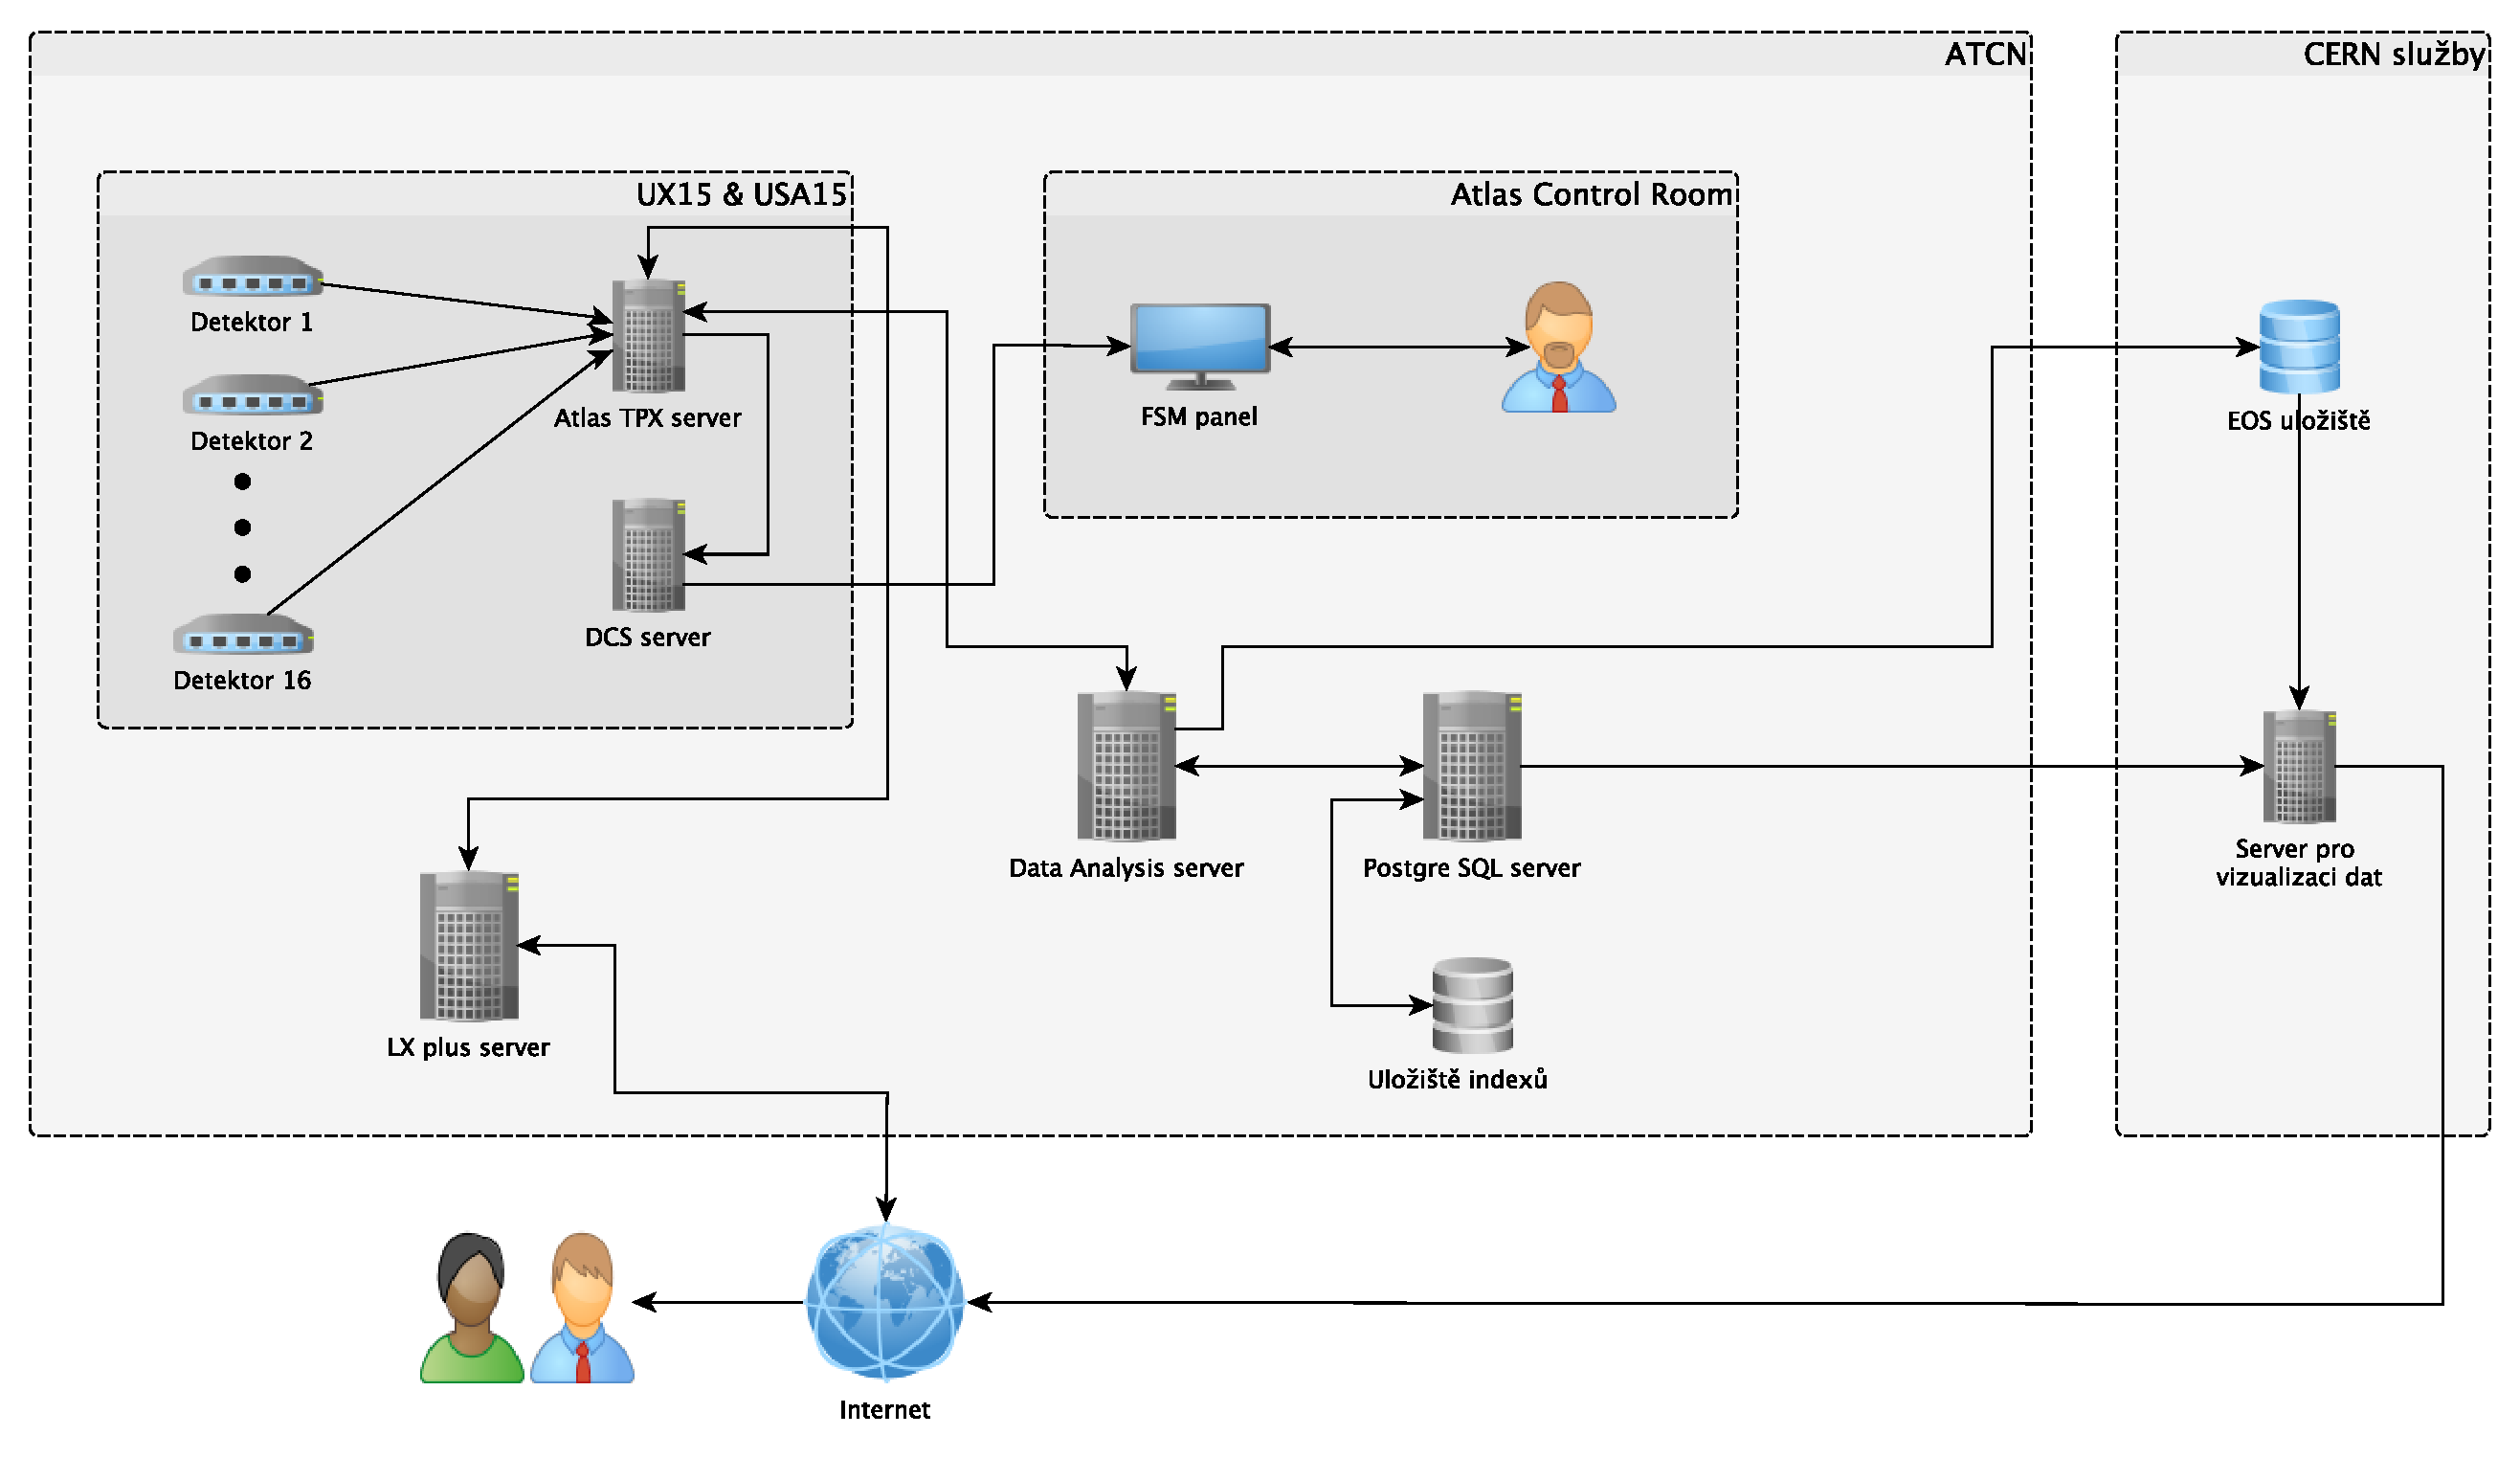
\includegraphics[width=16cm]{figures/atlas_tpx_sw_diagram.pdf}
		\caption{Atlas TPX - diagram softwarových komponent}
		\label{fig:tpx_sw_diagram}
	\end{center}
\end{figure}

\begin{description}
	\item[Popis architektury z pohledu řízení:] 
		Na obrázku \ref{fig:tpx_sw_diagram} se nachází Atlas TPX server, který je umístěn v serverové místnosti (USA15) Atlas experimentu, umístěné cca $100~m$ pod zemským povrchem. Tento server pomocí komunikačního protokolu (specifikovaném v \ref{atlas:cont:det}) řídí činnost detektorů (nastavování parametrů, ovládání akvizice apod.). Zároveň pomocí JSON REST API poskytuje rozhraní pro své řízení a předávání stavových informací (více v \ref{atlas:cont:api}). Díky tomuto rozhraní je možné činnost serveru řídit z ATCN sítě. Pro potřeby vzdáleného ovládání mimo síť ATCN slouží \texttt{LX plus server}, který zajistí spojení vytvořením SSH tunelu.\\
		Předávání stavových informací zajišťuje \texttt{DCS server}, který je od \texttt{Atlas TPX serveru} získává pomocí jeho API. Hlavním úkolem DCS je zajištění získávání stavových informací ze všech experimentů a detektorů homogenním způsobem a interakce s LHC (předávání dat luminozitě, stavu svazku urychlovače, radiační pozadí apod.). Tato data jsou dále předávána do Atlas Control Room, která se nachází na povrchu. Tam jsou tato data operátorů prezentována pomocí \texttt{FSM} panelu, což je aplikace, která vizualizuje stromovou strukturu všech systému a detektorů Atlas experimentu. Každý list této stromové struktury (detektor, senzor atd.) má několik proměnných, z nichž každá má předem definované intervaly s příslušnými stavy (\texttt{OK}, \texttt{WARNING}, \texttt{ERROR}, \texttt{FATAL} atd.). Výhodou této struktury je, že pokud kterýkoliv list změní svůj stav, tak se tato informace propaguje přes všechny nadřazené uzly, tudíž odhalení případné chyby je pro operátory mnohem snazší.
	\item[Popis architektury z pohledu analýzy a vizualizace dat:] 
		Když kterýkoliv detektor dokončí akvizici snímku, tak vygeneruje a pošle asynchronní událost \texttt{Atlas TPX serveru} s informací, že data jsou připravena k vyčtení. Následně server vyčte snímek z detektoru (i s jeho metadaty), zpracuje a připojí k němu informace o nastavení detektoru. Poté je třeba data přenést do \texttt{Data analysis serveru}, což v principu je možné dvěma\footnote{V současné době je možný pouze první způsob, protože díky politice CERNské síťové bezpečnosti a dlouhými schvalovacími termíny je Data analysis server a všechny s ním související systémy (web server, databáze s indexem a vlastní úložiště dat) prozatím umístěn v ÚTEF ČVUT v Praze.} způsoby:
		\begin{enumerate}
			\item \texttt{Atlas TPX server} uloží získaná data v textové podobě do lokálního (či síťového) datového úložiště, odkud jsou přenesena do \texttt{Data analysis serveru} pomocí automatického kopírovacího skriptu.
			\item Druhou možností je přenesení dat pomocí JSON REST API protokolu, který je \texttt{Data analysis serverem} implementován. Tento druhý způsob je výhodnější, neb minimalizuje prodlevu mezi dobou pořízení snímku a následném zpracováním \texttt{Data analysis serverem} a dostupnosti jeho vizualizace pomocí web serveru a zároveň přináší úsporu objemu přenesených dat.
		\end{enumerate}
		Hlavní úlohou \texttt{Data analysis serveru} je provedení tzv. Cluter analýzy. Jde o proces, při kterém jsou z každého snímku získány shluky sousedních pixelů (tzv. clusterů), které mají nenulovou hodnotu. Z těchto clusterů, resp. z jejich tvaru a celkové deponované energie částice (pokud zasažení pixely operovaly v TOT módu) je možné zjistit typ částice, která danou událost způsobila. Na obrázku \ref{fig:tpx_ca} můžete vidět 6 základních dělení clusterů, kde
		 \begin{enumerate}[label=(\alph*)]
			\item je tzv. \texttt{DOT}, způsobený fotony, či elektrony o energii do $10~keV$
			\item je tzv. \texttt{SMALL BLOB}, způsobený fotony, či elektrony s energií vetšinou nad $10~keV$
			\item je tzv. \texttt{CURLY TRACK}, způsobený elektrony do $10~MeV$
			\item je tzv. \texttt{HEAVY BLOBS}, způsobený těžce nabitými částicemi (na př. alfa)
			\item je tzv. \texttt{HEAVY TRACK}, způsobený těžce nabitými částicemi (na př. protony)
			\item je tzv. \texttt{STAIGHT TRACK}, způsobený těžce nabitými částicemi (muony apod.)
		\end{enumerate}
		Po dokončení analýzy dat, jsou data uložena do \texttt{ROOT}\footnote{\url{https://root.cern.ch/}} souborů (do souborové struktury po detektorech a hodinách). \texttt{ROOT} je framework, který je vyvíjen v CERN a je určený pro ukládání dat a jejich analýzu. Vygenerované soubory jsou ukládány do \texttt{EOS úložiště}, což je služba pro perzistentní ukládání \texttt{ROOT} souborů provozovaná CERN.\\
		Jelikož každý \texttt{ROOT} soubor má velikost řádově v jednotkách $GB$, jakékoliv operace nad nimi (na příklad vyhledávání) jsou velice časově náročné. Z tohoto důvodu vznikla \texttt{PostgreSQL} databáze s indexem na jednotlivé clustery, obsažené v \texttt{ROOT} souborech. 
		Pro vizualizaci dat slouží web server, který pomocí databáze s indexem a \texttt{ROOT} souborů poskytuje online výsledky cluster analýzy a další informace.
\end{description}

\begin{figure}[t]
	\begin{center}
		\includegraphics[width=10cm]{figures/ca.png}
		\caption{Cluster analýza - 6 základních typů clusterů (převzato z \cite{TurecekThesis2011})}
		\label{fig:tpx_ca}
	\end{center}
\end{figure}


%********************************************************************************
% Řídící software a jeho implementace
%********************************************************************************
\section{Řídící software a jeho implementace}\label{atlas:cont}
Tato kapitola je věnována návrhu a implementaci řídícího software sítě Atlas TPX, který je nasazen na Atlas TPX serveru (viz obr. \ref{fig:tpx_sw_diagram}). Úkolem  tohoto software se zajištění komunikace s detektory, zejména pak řízení akvizice, nastavování parametrů a vyčítání dat - tato komunikace bude popsána v kapitole \ref{atlas:cont:det}. Další úlohou tohoto software je poskytování rozhraní pro řízení své činnosti a pro předávání stavových informací o Atlas TPX síti. Toto rozhraní je implementováno pomocí \texttt{JSON REST API} a detailně bude popsáno v kapitole \ref{atlas:cont:api}. \todo

%********************************************************************************
% Řídící software a jeho implementace - Řízení detektorů
%********************************************************************************
\subsection{Řízení detektorů}\label{atlas:cont:det} % + komunikační protokol
Jak již bylo zmíně výše, detektor se skládá ze dvou \texttt{Timepix} detekčních čipů, \texttt{FPGA} a minipočítače \texttt{Raspberry Pi}, který implementuje komunikační protokol, díky kterému umožňuje řídícímu software ovládání činnosti detektoru. V podkapitole \ref{atlas:cont:det:comunikacni_protokol} naleznete popis tohoto komunikačního protokolu.

%********************************************************************************
% Řídící software a jeho implementace - Řízení detektorů
% > Komunikační protokol
%********************************************************************************
\subsubsection{Komunikační protokol}\label{atlas:cont:det:comunikacni_protokol}
Tabulka \ref{tab:com_packet} znázorňuje strukturu komunikačního rámce (tzv. paketu) tohoto protokolu pomocí posloupnosti bytů z pohledu Atlas TPX serveru, resp. z pohledu řídícího software. V horní části se nachází struktura odchozího paketu, kde:
\begin{description}
	\item[0x55]\footnote{\label{hexa}značení v hexadecimální soustavě} je tzv. \texttt{START BYTE}, který značí začátek paketu,
	\item[CMD] je typ příkazu (tzv. \texttt{COMMAND TYPE}) - viz tabulka přehledu příkazů \ref{tab:commands},
	\item[SIZE 1..4] je pole vždy o velikosti čtyřech bytů značících velikost (resp. počet bytů) položky \texttt{DATA}, zakódovaných v \texttt{BIG ENDIAN},
	\item[DATA 1 .. DATA n] je pole vlastních přenesených dat o velikosti $n$,
	\item[0xAA] \texttt{STOP BYTE}, který značí konec paketu.
\end{description}
Struktura odchozího paketu je velice podobná, až na byte \texttt{ERR}, který oproti příchozího paketu obsahuje. Tento byte může nabývat hodnoty 0x00 (když zpracování požadavku serveru detektorem proběhlo bet chyby), nebo 0x01 (jinak).

\begin{table}[th]
	\begin{center}
		\begin{bytefield}[bitwidth=1.35cm]{8}
			%\bitheader{0-8} \\
			\begin{rightwordgroup}{odchozí\\paket}
				\bitbox{1}{0x55} & \bitbox{1}{CMD} 
				& \bitbox{1}{SIZE 1} & \bitbox{1}{SIZE 2} & \bitbox{1}{SIZE 3} & \bitbox{1}{SIZE 4}
				& \bitbox{3}{DATA 1 .. DATA $n$} & \bitbox{1}{0xAA}
			\end{rightwordgroup} \\ \\ 
			%\bitheader{0-9} \\
			\begin{rightwordgroup}{příchozí\\paket}
				\bitbox{1}{0x55} & \bitbox{1}{CMD} & \bitbox{1}{ERR}
				& \bitbox{1}{SIZE 1} & \bitbox{1}{SIZE 2} & \bitbox{1}{SIZE 3} & \bitbox{1}{SIZE 4}
				& \bitbox{3}{DATA 1 .. DATA $n$} & \bitbox{1}{0xAA}
			\end{rightwordgroup}
			\end{bytefield}
	\end{center}
	\caption{Komunikační protokol - struktura paketů z pohledu serveru}
	\label{tab:com_packet}
\end{table}

\begin{table}[th]
	\begin{center}
		\begin{tabular}{|c|l|}
			\hline
			\textbf{Hodnota příkazu} & \textbf{Název příkazu} \\
			\hline
			0x01 & Ping \\
			\hline
			0x02 & Get status of the detector \\
			\hline
			0x03 & Reset of the device \\
			\hline
			0x04 & Set Bias and Timepix Clock \\
			\hline
			0x05 & Get Bias and Timepix Clock \\
			\hline
			0x06 & Set Pixel Configuration \\
			\hline
			0x07 & Get Pixel Configuration \\
			\hline
			0x08 & Set DAC \\
			\hline
			0x09 & Get DAC \\
			\hline
			0x0A & Perform Digital Test \\
			\hline
			0x0B & Perform Acquisition \\
			\hline
			0x0C & Readout Measured Data \\
			\hline
			0x0D & Direct FITPix Command \\
			\hline
			0x0E & Stop acquisition \\
			\hline
			0xFD & Asynchronous Event from device \\
			\hline
			0xFE & Reboot device \\
			\hline
			0xFF & Shut down \\
			\hline
			\end{tabular}
	\end{center}
	\caption{Komunikační protokol - přehled příkazů}
	\label{tab:commands}
\end{table}

%********************************************************************************
% Řídící software a jeho implementace - Řízení detektorů
% > Popis příkazů komunikačního protokolu
%********************************************************************************
\subsubsection{Popis příkazů komunikačního protokolu}
Následuje struční popis příkazů komunikačního protokolu z pohledu obsahu vlastních přenesených dat odchozího a příchozího paketu (viz tabulka \ref{tab:com_packet})

\begin{description}
	\item[0x01 - Ping]:
		Příkaz pro ověření spojení s detekorem. Na základě rozdílu času odeslání a přijetí paketu je vypočtena prodleva spojení v $ns$ (tzv. ping)
		\begin{description}
			\item[Odchozí data:] nic
			\item[Příchozí data:] nic
		\end{description}
	\item[0x02 - Get status of the detector]:
		Příkaz pro zjištění stavu detektoru.	
		\begin{description}
			\item[Odchozí data:] nic
			\item[Příchozí data ($2~B$):] GST MST
				\begin{itemize}
					\item GST - General Status (obecný status)
						\begin{itemize}
							\item 0x00 - Ok
							\item 0x01 - Chyba detekčního čipu
							\item 0x02 - Obecná chyba
						\end{itemize}
					\item MST - Measurement Status (měřící status)
						\begin{itemize}
							\item 0x00 - Nečinný
							\item 0x01 - Probíhá akvizice
							\item 0x02 - Čekání na trigger
							\item 0x03 - Data připravena k vyčtení
							\item 0x04 - Chyba akvizice
						\end{itemize}
				\end{itemize}
		\end{description}
	\item[0x03 - Reset of the device]:
		Tento příkaz slouží pro vyresetování \texttt{FPGA} a dalších řídících struktur detektoru.
		\begin{description}
			\item[Odchozí data:] nic
			\item[Příchozí data:] nic
		\end{description}
	\item[0x04 - Set Bias and Timepix clock]:
		Příkaz nastavující napětí (Bias) na obou Timepix čipech a jejich meřící frekvenci (Timepix clock)
		\begin{description}
			\item[Odchozí data ($24~B$):] BIAS1($8~B$) BIAS2($8~B$) CLK($8~B$)
				\begin{itemize}
					\item BIAS1, BIAS2 - hodnota napětí pro Timepix čipy (zakódovaná jako 64-bitové double-precision číslo dle standartu \texttt{IEEE 754})
					\item CLK - Měřící frekvence obou Timepix čipů (zakódovaná jako 64-bitové double-precision číslo dle standartu \texttt{IEEE 754})
				\end{itemize}
			\item[Příchozí data:] nic
		\end{description}
	\item[0x05 - Get Bias and Timepix clock]:
		Příkaz pro vyčtení úrovně napětí z obou Timepix čipů a jejich meřící frekvenci
		\begin{description}
			\item[Odchozí data:] nic
			\item[Příchozí data ($24~B$):] BIAS1($8~B$) BIAS2($8~B$) CLK($8~B$)
				\begin{itemize}
					\item BIAS1, BIAS2 - hodnota napětí pro Timepix čipy (zakódovaná jako 64-bitové double-precision číslo dle standartu \texttt{IEEE 754})
					\item CLK - Měřící frekvence obou Timepix čipů (zakódovaná jako 64-bitové double-precision číslo dle standartu \texttt{IEEE 754})
				\end{itemize}
		\end{description}
	\item[0x06 - Set Pixel Configuration]:
		Příkaz pro nastavení konfigurace pro každý pixel detektoru
		\begin{description}
			\item[Odchozí data ($(1+(65536~nebo~2*65536))~B$):] TYPE($1~B$) PIXCFG($(65536~nebo~2*65536)~B$)
				\begin{itemize}
					\item TYPE - Výběr čipu, pro který je konfigurace určena
						\begin{itemize}
							\item 0x00 - Konfigurace určena oboum čipům (délka PIXCFG je $2*65536~B$)
							\item 0x01 - Konfigurace určena prvnímu čipu (délka PIXCFG je $65536~B$)
							\item 0x02 - Konfigurace určena druhému čipu (délka PIXCFG je $65536~B$)
						\end{itemize}
					\item PIXCFG - Pole konfiguračních bytů (každý byte je pro jeden pixel) pro jednotlivé pixely. Délka tohoto pole je závyslá na parametru TYPE. Struktura bytu pro konfiguraci pixelu je následovná: \\ MASK\_BITE($1~b$) TEST\_BITE($1~b$) THL($4~b$) MODE($2~b$)
						\begin{itemize}
							\item MASK\_BITE - Pixel je aktivní při hodnotě $1$, zamaskovaný při $0$.
							\item TEXT\_BITE - \todo
							\item THL - Tyto čtyři bity udávají číslo od 0 do 15, které je použito pro posun globální hodnoty THL
							\item MODE - Mód pixelu (0 - Medipix, 1 - Time-Over-Treshold, 2 One-Hit, 3 - Time-of-Arrival)
						\end{itemize}
				\end{itemize}
			\item[Příchozí data:] nic
		\end{description}
	\item[0x07 - Get Pixel Configuration]:
		Příkaz pro vyčtení konfigurace pixelů detektoru.
		\begin{description}
			\item[Odchozí data ($1~B$):] TYPE - Výběr čipu, pro který je konfigurace určena (viz předchozí příkaz)
			\item[Příchozí data ($(65536~nebo~2*65536)~B$):] PIXCFG (viz předchozí příkaz)
		\end{description}
	\item[0x08 - Set DAC]:
		Příkaz pro nastavení hodnot DAC převodníků detektoru.
		\begin{description}
			\item[Odchozí data ($3~B$):] DAC\_IDX DAC\_VAL DAC\_VAL
				\begin{itemize}
					\item DAC\_IDX - DAC index
					\item DAC\_VAL - DAC hodnota
				\end{itemize}
			\item[Příchozí data:] nic
		\end{description}
	\item[0x09 - Get DAC]:
		Příkaz pro vyčtení hodnoty DAC převodníků detektoru.
		\begin{description}
			\item[Odchozí data ($1~B$):] DAC\_IDX
				\begin{itemize}
					\item DAC\_IDX - DAC index
				\end{itemize}
			\item[Příchozí data ($2~B$):] DAC\_VAL DAC\_VAL
				\begin{itemize}
					\item DAC\_VAL - DAC hodnota
				\end{itemize}
		\end{description}
	\item[0x0A - Perform Digital Test]:
		Příkaz pro vykonání testu digitálních částí detektoru.
		\begin{description}
			\item[Odchozí data:] nic
			\item[Příchozí data ($3~B$):] BPC BPC BPC
				\begin{itemize}
					\item BPC - Počet chybných pixelů detektoru
				\end{itemize}
		\end{description}
	\item[0x0B - Perform Acquisition]:
		Příkaz pro zahájení akvizice snímku/snímků.
		\begin{description}
			\item[Odchozí data ($13~B$):] ACQTM($8~B$) ACQCNT($4~B$) TGRMOD
				\begin{itemize}
					\item ACQTIM - Akviziční čas v sekundách (zakódovaný jako 64-bitové double-precision číslo dle standartu \texttt{IEEE 754}).
					\item ACQCNT - Počet snímku (pokud je 0, detektor bude opakovat akvizici s těmito parametry až do její zastavení)
					\item TRIGMOD - Mód triggeru
						\begin{itemize}
							\item 0x00 - bez triggeru
							\item 0x01 - akvizice zahájena na signál triggeru
							\item 0x02 - akvizice ukončena
							 na signál triggeru
						\end{itemize}
				\end{itemize}
			\item[Příchozí data:] nic
		\end{description}
	\item[0x0C - Read Measured Data]:
		Tento příkaz slouží pro vyčtení naměřených dat z detektoru.
		\begin{description}
			\item[Odchozí data ($6~B$):] DET TYPE FRAME\_ID FRAME\_ID FRAME\_ID FRAME\_ID
				\begin{itemize}
					\item DET - selektor Timepix čipu
						\begin{itemize}
							\item 0x00 - oba čipy
							\item 0x01 - jen první čip
							\item 0x02 - jen druhý čip
						\end{itemize}
					\item TYPE - typ vyčítaných dat
						\begin{itemize}
							\item 0x00 - deserializovaný a derandomizovaný snímek
							\item 0x01 - surová data z FPGA
							\item 0x02\_ID - metadata k danému snímku (akviziční čas, napětí apod.)
						\end{itemize}
					\item FRAME\_ID - ID naměřeného snímku
				\end{itemize}
			\item[Příchozí data:] Velikost a typ příchozích dat se liší dle použitých parametrů DET a TYPE
				\begin{itemize}
					\item Pro TYPE 0x00 přijde pole bytů hodnot čítačů jednotlivých pixelů (hodnota každého pixelu je reprezentována pomocí dvou bytů)
					\item Pro TYPE 0x01 přijdou blíže nespecifikovaná surová data z FPGA
					\item Pro TYPE 0x02 přijdou metadata, vázající se k danému snímku s následující strukturou:
						\begin{itemize}
							\item UNIX časové razítko začátku akvizice [$ms$] ($5~B$)
							\item Bias1 - měřící napětí prvního čipu [$V$] ($8~B$, double-precision dle \texttt{IEEE 757})
							\item Bias2 - měřící napětí druhého čipu [$V$] ($8~B$, double-precision dle \texttt{IEEE 757})
							\item Měřící frekvence [$Hz$] ($8~B$, double-precision dle \texttt{IEEE 757})
							\item Doba akvizice [$s$] ($8~B$, double-precision dle \texttt{IEEE 757})
						\end{itemize}	

				\end{itemize}
		\end{description}
	\item[0x0D - Direct FPGA Command]:
		Příkaz pro přímé poslání dat do FPGA a získání odpovědi.
		\begin{description}
			\item[Odchozí data:] Dle použitého příkazu
			\item[Příchozí data:] Dle použitého příkazu
		\end{description}
	\item[0x0E - Stop acquisition]:
		Příkaz pro zastavení aktuálně probíhající akvizice.
		\begin{description}
			\item[Odchozí data ($1~B$):] TYPE
				\begin{itemize}
					\item TYPE: Typ zastavení
						\begin{itemize}
							\item 0x00 - Zastavení akvizice po dokončení aktuálně pořizovaného snímku
							\item 0x01 - Bezprostřední zastavení akvizice 
						\end{itemize}
				\end{itemize}
			\item[Příchozí data:] nic
		\end{description}
	\item[0xFD - Asynchronous Event From Device]:
		Tento typ příkazu je asynchronní a detektor ho posílá samovolně dle nastalé události - na příklad dokončení akvizice.
		\begin{description}
			\item[Příchozí data ($5~B$):] EVID VAL VAL VAL VAL
				\begin{itemize}
					\item EVID - Typ nastalé události (na př. 0x00 pro událost dokončení akvizice)
					\item VAL - Doplňující data (na př. ID snímku pro událost dokončení akvizice)
				\end{itemize}
		\end{description}
	\item[0xFE - Reboot of the Device]:
		Příkaz pro restartování detektoru.
		\begin{description}
			\item[Odchozí data:] nic
			\item[Příchozí data:] nic
		\end{description}
	\item[0xFF - Shutdown of the Device]:
		Příkaz pro vypnutí detektoru.
		\begin{description}
			\item[Odchozí data:] nic
			\item[Příchozí data:] nic
		\end{description}
\end{description}


%********************************************************************************
% Řídící software a jeho implementace - Řízení detektorů
% > Synchronní a asynchronní příkazy komunikačního protokolu
%********************************************************************************
\subsubsection{Synchronní a asynchronní příkazy komunikačního protokolu}\label{atlas:com:synchonni_a_asynchonni_prikazy}
Téměř všechny příkazy komunikačního protokolu jsou synchronní, tzn. server vyšle odchozí paket (s typem příkazu a jeho daty), který detektor zpracuje a bezprostředně vygeneruje a pošle odchozí paket (s příslušnými daty, typem příkazu a informací, zda-li při jeho zpracování došlo k chybě). Příkladem této synchronní komunikace je příkaz ping na obrázku \ref{fig:uml:com_priklad} nahoře.

Vedle synchronních příkazů existuje i jeden asynchronní - \texttt{0xFD - Asynchronous Event From Device}. V současné verzi komunikačního protokolu je tento příkaz využit jen pro oznámení serveru, že detektor dokončil akvizici a má data připravena k vyčtení.

Na obrázku \ref{fig:uml:com_priklad} je znázorněn příklad kombinace synchronní a asynchronní komunikace pro pořízení snímku. Nejprve server vyšle synchronní příkaz s žádostí o provedení akvizice (s parametry: doba akvizice, počet snímků a mód triggeru) na který hned dostane odpověď. Následuje vyčítací smyčka - detektor udělá akvizici snímku (pokud již všechny neudělal) a vyšle serveru asynchronní příkaz s kódem právě dokončené akvizice a s ID\footnote{unikátní číslo snímku od spuštění detektoru} snímku. Tuto asynchronní zprávu server zachytí a provede vyčítací sekvenci (pomocí příkazu \texttt{0x0C - Read Measured Data}), jejíž kroky se mohou lišit dle konfigurace. Ve výchozím nastavení tato sekvence vypadá následovně:
\begin{enumerate}
	\item Vyčtení vlastního snímku (hodnot jednotlivých pixelů).
	\item Vyčtení metadat (tzv. \texttt{DSC}). Tato data obsahují dodatečné informace ke snímku, jako na příklad přesnou dobu akvizice, čas začátku akvizice a měřící napětí a frekvenci Timepix čipů.
\end{enumerate}

\begin{figure}[t]
	\begin{center}
		\begin{sequencediagram}
			\newinst{s}{:AtlasTPX server}
			\newinst[7]{d}{:Detektor}
			\begin{sdblock}{Ping}{}
				\begin{call}{s}{ping()}{d}{}
				\end{call}
			\end{sdblock}
			\begin{sdblock}{Pořízení snímku}{}
				\begin{call}{s}{performAcq(framesCount, acqTime, trigMod)}{d}{return(success)}	
				\end{call}
				%\postlevel
				\begin{sdblock}{Měřící smyčka}{while(currentFrame <= framesCount)}
					\begin{callself}{d}{performAcq}{acqFinished}
					%\postlevel	
					\end{callself}
					\mess{d}{asynchronousEvent - acq finished}{s}
					%\postlevel
					\begin{call}{s}{readOutMeasuredData(det, frameID, type = FRAME)}{d}{return(data)}
					\end{call}
					%\postlevel
					\begin{call}{s}{readOutMeasuredData(det, frameID, type = DSC)}{d}{return(data)}
					\end{call}
				\end{sdblock}
			\end{sdblock}
		\end{sequencediagram}
		\caption{Příklad použití komunikačního protokolu}
		\label{fig:uml:com_priklad}
	\end{center}
\end{figure}


%********************************************************************************
% Řídící software a jeho implementace - Řízení detektorů
% > Implementace modulu pro řízení detektorů na straně serveru
%********************************************************************************
\subsubsection{Implementace modulu pro řízení detektorů na straně serveru}\label{atlas:cont:impl}
V této podkapitole bude popsána implementace řízení detektorů v řídícím softwaru sítě Atlas TPX. Celý software byl implementován v jazyce \texttt{JAVA} za pomoci build nástroje \texttt{Maven}\footnote{\url{https://maven.apache.org/}} a knihoven \texttt{Dropwizard}\footnote{\url{http://www.dropwizard.io}}, \texttt{Retrofit}\footnote{\url{http://square.github.io/retrofit/}} a \texttt{RxJava}\footnote{\url{https://github.com/ReactiveX/RxJava}}.

Jak již bylo zmíněno výše, detektory jsou připojeny k Atlas TPX serveru přes ethernetové rozhraní a pomocí TPC/IP protokolu je vlastní komunikace realizována pomocí výše popsaného komunikačního protokolu. Z pohledu navazování spojení byla použita architektura klient-server tak, že detektor plní roli serveru a Atlas TPX server zase klienta. Tato architektura bylo použita s ohledem na robustnost a stabilitu této sítě a aby úloha navazování spojení zůstala v kompetenci Atlas TPX serveru. Když by na příklad došlo k přerušení napájení nebo jiné chybě jednoho z detektorů, Atlas TPX server by nebyl schopen se pokusit o znovu navázání spojení.

\begin{figure}[th]
	\begin{center}
		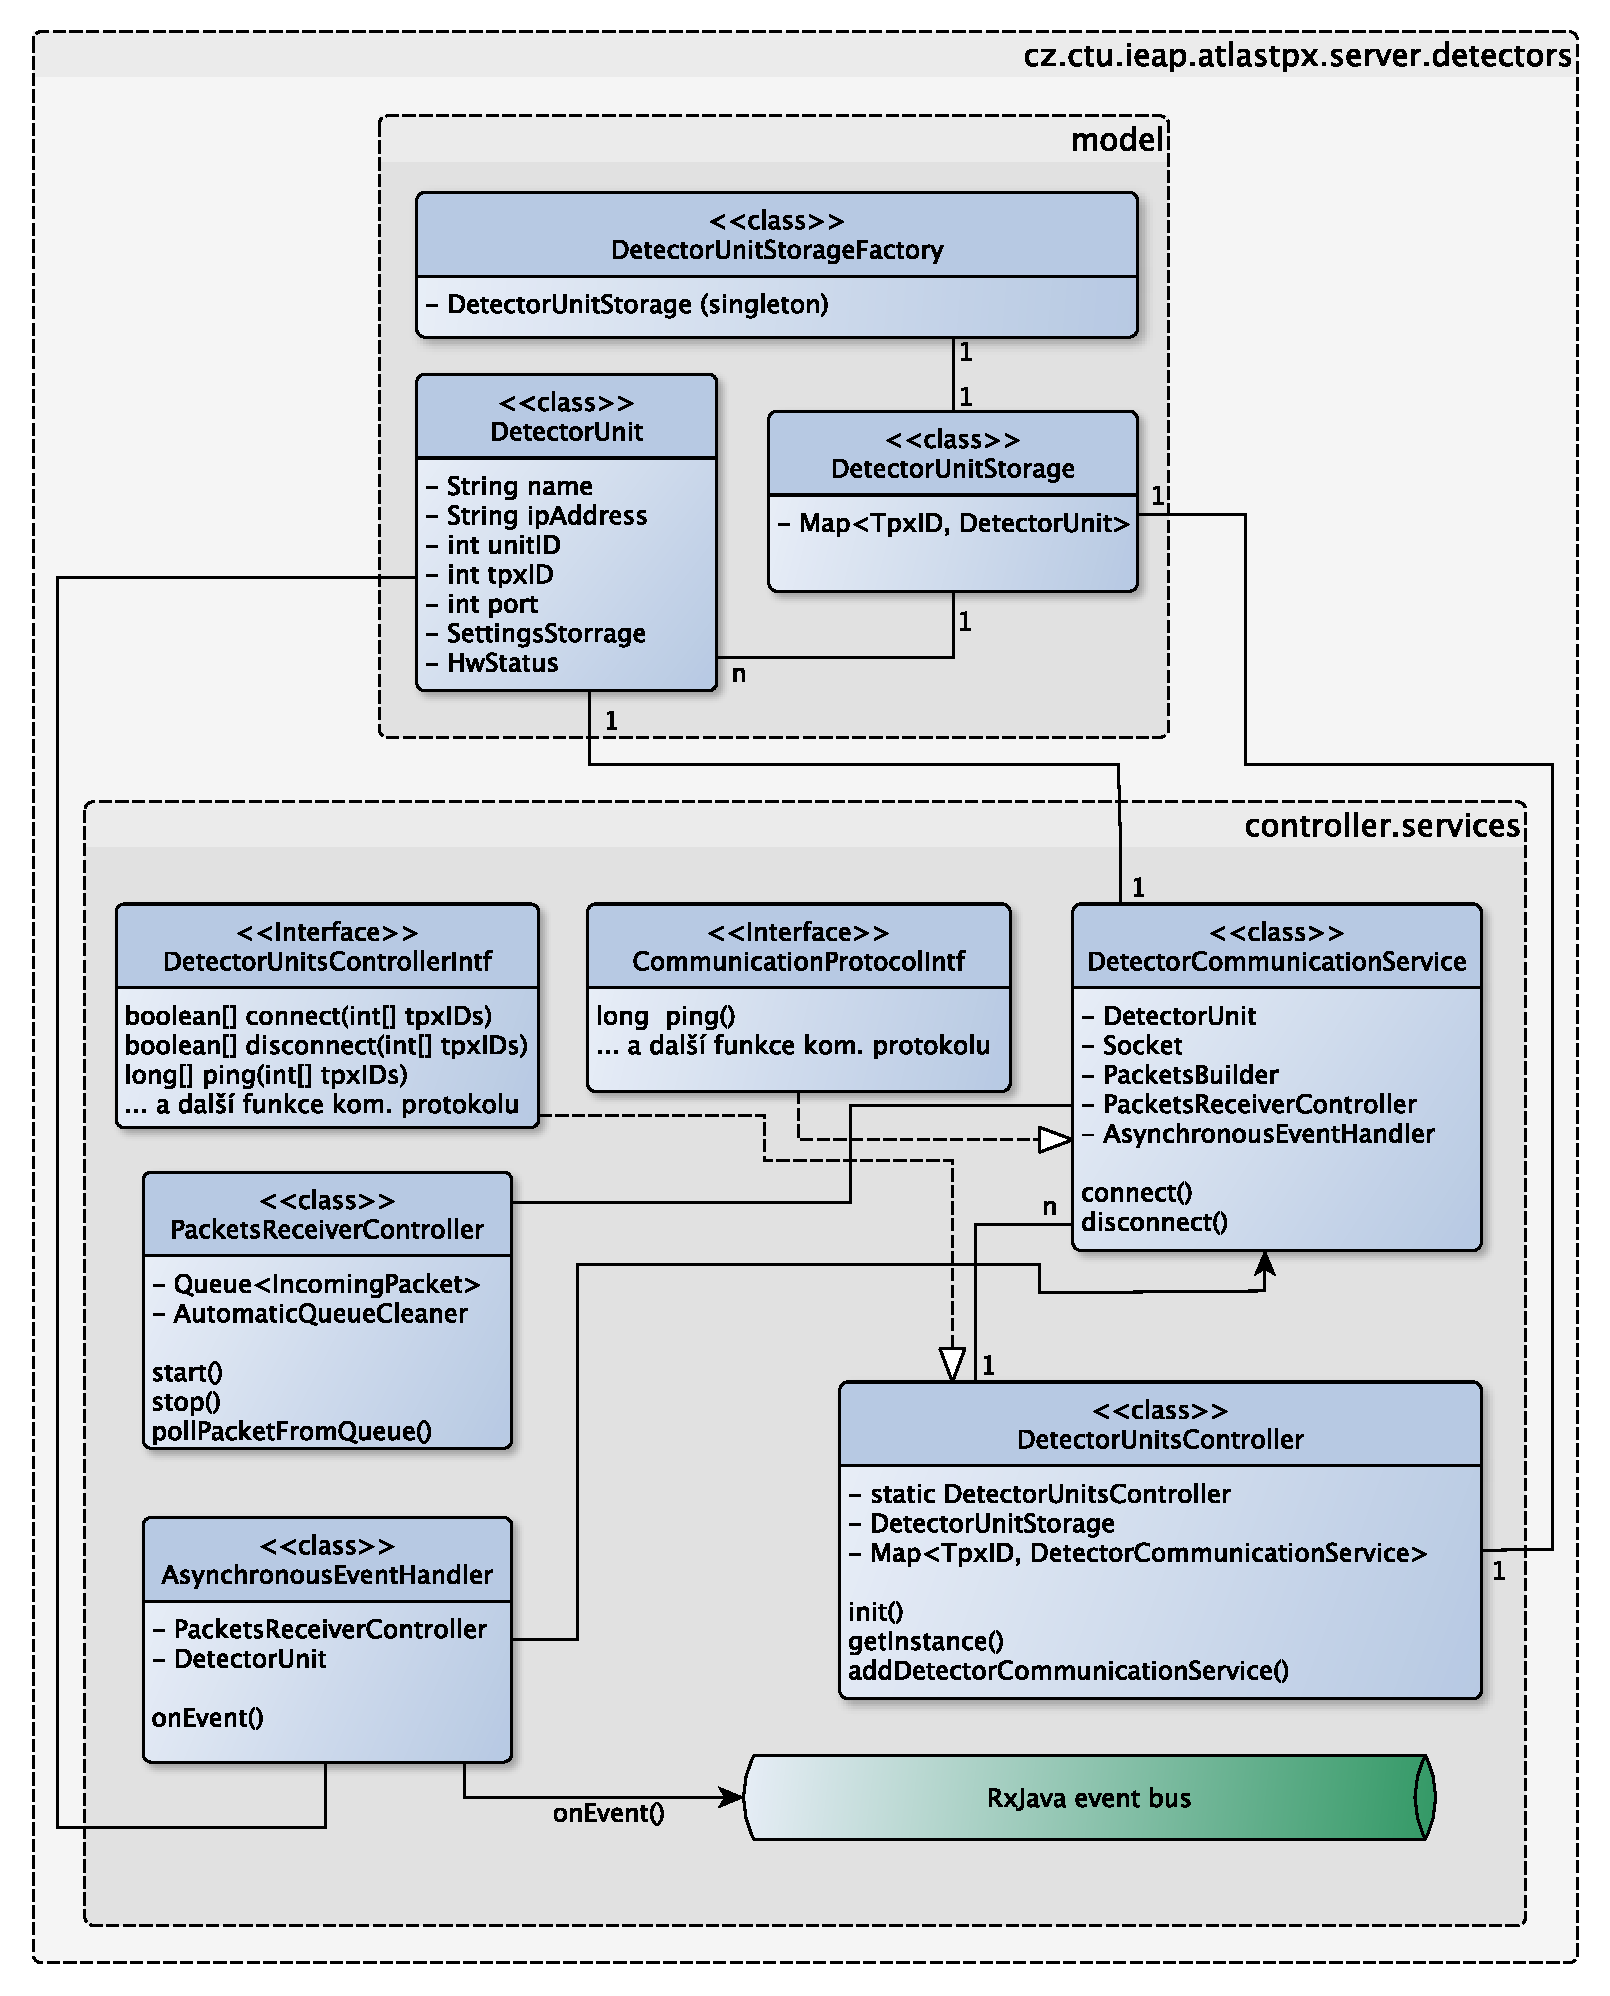
\includegraphics[width=11cm]{figures/atlas_tpx_detectors_class.pdf}
		\caption{Diagram tříd modulu pro ovládání detektorů}
		\label{fig:class:detectors}
	\end{center}
\end{figure}

Na obrázku \ref{fig:class:detectors} můžete vidět diagram tříd modulu pro práci s detektory řídícího softwaru. Tento diagram není úplný a obsahuje jen několik nejdůležitějších tříd, zbytek je k nalezení na přiloženém CD.

Při návrhu tohoto modulu bylo vycházeno z návrhového vzoru Model-View-Controller \cite{DesignPatterns-Gamma:1995:DPE:186897}, resp. z jeho modifikace Model-Controller, protože tento modul žádnou prezentační vrstvu nemá. 

Začněme popisem balíčku \texttt{model}. Jeho nejdůležitější třídou je třída \texttt{DetectorUnit}, která uchovává všechny informace o jednom detektoru, jako na příklad název, tpxID, unitID, ip adresu, port, \texttt{SettingsStorage} (úložiště nastavení detektoru, jako na příklad bias, clock, parametry akvizice, DAC hodnoty atd.) a \texttt{HwStatus} (tento objekt nese informace o posledních naměřeních údajích získaných z detektoru, jako třeba aktuální hodnoty bias, ping, obecný a měřící status apod.).

Pro uchovávání všech instancí třídy \texttt{DetectorUnit} slouží singleton \cite{DesignPatterns-Gamma:1995:DPE:186897} třída \texttt{DetectorUnit\\Storage}, která tyto instance uchovává v kolekci HashMap, jejímž klíčem je TpxID (Integer). Instanci tohoto singletonu je možné získat pomocí třídy \texttt{DetectorUnitStorageFactory}, resp. pomocí její statické metody \texttt{getStorage()}. Před prvním použití je třeba nejprve toto úložiště inicializovat pomocí statické metody \texttt{DetectorUnitStorageFactory.initStorage(String\\initFilePath)}, které se coby parametr předá cesta v souborovém systému k "*.csv" souboru s tabulkou s detektory. Každý řádek tohoto souboru reprezentuje jeden detektor a je v následujícím formátu:
\begin{center}
	název\_detektoru\textbf{\Large{;}}ip\_adresa\textbf{\Large{;}}unit\_id\textbf{\Large{;}}tpx\_id\textbf{\Large{;}}port
\end{center}

V balíčku \texttt{controller.services} se nachází vlastní logika tohoto modulu. 
Třída \texttt{Detector\\CommunicationService} se stará o vlastní komunikaci s detektorem (jedna instance = jeden detektor). Tato třída obsahuje instanci třídy \texttt{DetectorUnit} (předané v konstruktoru), která mimo jiné obsahuje IP adresu a port příslušného detektoru. Tyto parametry se používají v metodě \texttt{connect()}, ve které se vytvoří spojení s detektorem (socket, BufferedOutputStream, BufferedInputStream apod.). Pro odpojení detektoru zase slouží metoda \texttt{dicconnect()}. Krom metod pro síťovou komunikaci obsahuje i všechny metody implementované z interface \texttt{CommunicationProtocolIntf} - všechny synchronní metody komunikačního protokolu. 

Pro příjem příchozích paketů z detektoru vznikl \texttt{PacketsReceiverController}. Ten ve vlastním vlákně vyčítá proud bytů, přicházejících z detektoru a následně provádí jejich parsování, jehož výsledkem je instance objektu \texttt{IncomingPacket}, které obsahuje typ příkazu, příznak chyby a vlastní data. Takto vzniklý paket je zařazen do fronty příchozích paketů detektoru (implementované jako \texttt{ConcurrentLinkedQueue<IncomingPacket>}). Nad touto frontou pracují jednak všechny metody se synchronními příkazy komunikačního protokolu (které sledují, zda-li se v ní v daném časovém intervalu objeví odpověď), ale také instance objetu \texttt{AsynchronousEventHandlerController}. Ten ve vlastním vlákně tuto frontu sleduje a objeví-li se paket s typem příkazu \texttt{0xFD (Asynchronous Event From Device)}, tak ho z fronty odebere, jeho vlastní data rozparsuje a dále zpracuje. Pokud se na příklad jedná o událost dokončené akvizice, tak \texttt{ReadOutService} snímek z detektoru vyčte a pomocí \texttt{RxJava event bus} vyšle asynchronní zprávu napříč celou aplikací s vyčteným snímkem. Zde byl použit návrhový vzor Producer - Consumer, kde \texttt{AsynchronousEventHandlerController} představuje Producer a na kterémkoliv jiném místě aplikace se Consumer (možno i více Consumerů) muže zaregistrovat ke sledování událostí v event bus. Příkladem takového Comsumera může být \texttt{FrameSaverController}, který se postará o uložení získaného snímku (viz kapitola \ref{atlas:cont:output}).

Aby bylo možné pohodlně ovládat více detektorů současně, vznikl\\\texttt{DetectorUnitsController}. Ten implementuje interface \texttt{DetectorUnitsControllerIntf}, jehož metody pokrývají veškerou funkcionalitu detektoru, jako třeba metody k navázání a ukončení spojení, ale také všechny metody komunikačního protokolu. Všechny tyto metody mají jeden společní parametr - \texttt{int[] tpxIDs} (pole TpxID detektorů). Tento parametr určuje, nad kterými detektory se má daná metoda hromadně vykonat. Jejich výstupem je zase pole, jehož typ se liší dle příkazu (na příklad pro metodu connect je to pole boolean proměnných - značící úspěch připojení, pro ping zase double čísel, udávajících odezvu spojení v $ns$). Tento objekt je zase typu singleton a jeho instanci lze získat pomocí metody \texttt{getInstance()}. Po spuštění aplikace je však třeba tento singleton nainicializovat pomocí metody \texttt{init()}, která pomocí \texttt{DetectorUnitStorageFactory} vytvoří datovou strukturu  s \texttt{DetectorCommunicationService} jednotlivých detektorů.


%********************************************************************************
% Řídící software a jeho implementace - Řízení detektorů
% > Emulátor detektoru
%********************************************************************************
\subsubsection{Emulátor detektoru}
Pro účely vývoje a testování řídícího software pro \texttt{Atlas TPX server} byl vyvinut emulátor detektoru, který plně emuluje jeho činnost. Emulátor byl rovněž napsán v jazyce \texttt{JAVA} a jeho zdrojové kódy a spustitelný \texttt{jar} soubor naleznete na přiloženém CD.

Emulátor se spouští se dvěma povinnými parametry, kde
\begin{enumerate}
	\item je port, na kterém server emulátoru naslouchá (celé číslo),
	\item je pravděpodobnost, s jakou při zpracovávání požadavku bude simulována chyba - $0$ znamená bez chyb, $1$ samé chyby (desetinné číslo).
\end{enumerate}

\begin{figure}[t]
	\begin{center}
		\begin{sequencediagram}
			\newinst{ss}{:AtlasPix (ServerSocket)}
			\newthread[blue]{ch}{:ClientHandler}
			\newthread[gray]{pr}{:PaketReceiver}
			\newthread[red]{ap}{:AcquisitionPerformer}
			\begin{sdblock}{Připojení klienta}{}
				\begin{call}{ss}{acceptClient}{ch}{success}
					\begin{call}{ch}{startReceiving}{pr}{success}
					\end{call}
				\end{call}
			\end{sdblock}
			\begin{sdblock}{Akvizice snímku}{}
				\begin{callself}{pr}{performAcqRequest}{success}
					\begin{call}{pr}{acqRequest}{ch}{success}
						\mess{ch}{performAcq}{ap}
					\end{call}	
				\end{callself}	
				\postlevel
				\mess{ap}{onAcqPerformed}{ch}
				\begin{callself}{ch}{onAcqPerformed}{success}
				\end{callself}	
			\end{sdblock}			
		\end{sequencediagram}
		\caption{Emulátor detektoru - sekvenční diagram připojení klienta a pořízení snímku}
		\label{fig:uml:emulator}
	\end{center}
\end{figure}

Na obrázku \ref{fig:uml:emulator} je zobrazen sekvenční diagram dvou případů užití tohoto emulátoru. První případ užití znázorňuje připojení klienta (na př. \texttt{Atlas TPX serveru}) a druhý pak proces zpracování žádosti o snímek a jeho vygenerování.

Pojďme si nyní popsat první část - připojení klienta. Ve třídě \texttt{AtlasPix}, resp. v její metodě \texttt{startServer()} se nachází nekonečná smyčka, ve které je pomocí instance třídy \texttt{ServerSocket} navázáno spojení s novými klienty. Když spojení s klientem je navázáno, je vytvořen klientský socket, pomocí kterého dojde v vytvoření instance třídy \texttt{ClientHandler}. Ta se v samostatném novém vláknu stará o obsluhu nově připojeného klienta. Zároveň \texttt{ClientHandler} vytvoří instanci třídy \texttt{PaketReceiver}, který čte proud bytů přijatých od klienta a parsuje jej do objektů typu \texttt{IncomingPacket}.

Tím se dostáváme k druhému příkladu případu užití - akvizici snímku. Poté, co \texttt{PaketReceiver} přijme nový paket, tak ho vloží do fronty paketů. Tuto frontu z druhé strany čte a zpracovává \texttt{ClientHandler}. Všechny příchozí pakety od klienta mohou obsahovat jen synchronní příkazy komunikačního protokolu, takže může být okamžitě nasimulován příslušný stav emulátoru a vygenerována odpověď klientovi. 

V našem případe akvizice snímku je situace trochu složitější. \texttt{PaketReceiver} odchytí nový paket, obsahující žádost o provedení akvizice, který předá do fronty příchozích paketů. Když se \texttt{ClientHandler} dostane k jeho zpracování, tak vytvoří objekt typu \texttt{AcquisitionRequest} a předá ho instanci třídy \texttt{AcquisitionPerformer}. Ten žádost o akvizici zařadí do příslušní fronty, kde čeká, až samostatné akviziční vlákno se dostane k jejímu zpracování. Při zpracovávání žádosti o akvizici je vygenerováno náhodná matice hodnot pixelů (o velikosti $256\times512$) a také příslušná metadata, jako na příklad akviziční čas, bias obou čipů (s přičtenou náhodnou veličinou, simulující fluktuaci napětí na křemíkovém povrchu detekčních čipů) apod. Po vygenerování těchto hodnot se akviziční vlákno uspí na dobu akvizice, aby se chování emulátoru co nejvíce přiblížilo skutečnému detektoru.

Následně je připojenému klientovi poslána asynchronní zpráva o dokončené akvizici. Tato zpráva obsahuje příznak, že naměřená data jsou připravena k vyčtení a také ID vygenerovaného snímku. 

Poté klient pošle příkaz pro vyčtení naměřených dat (resp. dva příkazy - jeden pro vlastní snímek a druhý pro metadata), což bylo popsáno v kapitole \ref{atlas:com:synchonni_a_asynchonni_prikazy} - viz obr. \ref{fig:uml:com_priklad}.

%********************************************************************************
% Řídící software a jeho implementace - REST API server
%********************************************************************************
\subsection{REST API server}\label{atlas:cont:api}
Řídící software se svému ovládání poskytuje rozhraní přes \texttt{JSON REST\footnote{z angl. Representational State Transfer} API}. Pro toto rozhraní byla použita knihovna Dropwizard\cite{dropwizard}, která vznikla složením několika dalších knihoven, zejména pak:
\begin{description}
	\item[Jetty] je open-source software, v současné době vyvíjen Eclipse Foundation. Tato knihovna obsahuje Java HTTP webový server, který na rozdíl od běžných webových serveru (které vetšinou přes HTTP protokol poskytují soubory koncovým uživatelům) byl navržen pro strojově orientovanou komunikaci.
	\item[Jersey] je open-source knihovna (která dle \cite{dropwizard} vychází z \texttt{JAX-RS}\footnote{\url{http://jcp.org/en/jsr/detail?id=311}}) a byla použita pro zajištění REST API. Tato knihovna umožňuje elegantně pomocí anotací mapovat HTTP dotazy na jednoduché Java objety.
	\item[Jackson] je výkonný nástroj pro práci s \texttt{JSON}\footnote{JSON je v dnešní době standardem pro zápis a výměnu strukturovaných, člověkem i strojem čitelných dat.} objekty v jazyce Java. Tato knihovna umožňuje ergonomicky mapovat data v JSON do Java objektů pomocí anotací.
\end{description}

V této podkapitole bude popsána implementace této knihovny do \texttt{Atlas TPX serveru} a její provázanost na modul pro řízení detektorů (\ref{atlas:cont:impl}).

%********************************************************************************
% Řídící software a jeho implementace - REST API server
% > Konfigurace a spuštění serveru
%********************************************************************************
\subsubsection{Konfigurace a spuštění serveru}
Server je možné spustit z příkazové řádky pomocí příkazu \texttt{"java -jar atlasTpxServer.jar server config.yml"}, kde \texttt{atlasTpxServer.jar} je spustitelný binární soubor serveru, \texttt{server} je povinný parametr (znamenající spuštění programu v módu server) a \texttt{config.yml}, což je také povinný parametr, udávající cestu v souborovém systému ke konfiguračnímu souboru serveru.

V příloze \ref{app:config} strukturu tohoto konfiguračního souboru, ve kterém je možné nastavit následující:
\begin{description}
	\item[Umístění tabulky s detektory] (detectorsConfigPath - viz \ref{app:config} řádek 8)\\
		Tento parametr udává cestu v souborovém systému ke konfiguračnímu "*.csv" souboru, obsahující tabulku všech detektoru a jejich parametrů, popsanou v \ref{atlas:cont:impl}.
	\item[Nastavení webového serveru] (server - viz \ref{app:config} řádek 11)\\
		V rámci tohoto objektu je možné nastavit použitý typ protokolu spojení (\texttt{HTTP}/\texttt{HTTPS}), port, počty vláken a další.
	\item[Logování] (logging - viz \ref{app:config} řádek 30)\\
		Pomocí tohoto parametru je možné nastavit úroveň a cíl vytvářených logů. V přiloženém konfiguračním souboru bylo použito dvojího logování a to na standardní výstup a do souboru (oba úrovně \texttt{INFO}). Při logování do souboru je možné navíc nastavit automatickou archivaci.
	\item[Automatické vyčítání snímků] (readOutDataAutomatically - viz \ref{app:config} řádek 54)\\
		Tento parametr typu \texttt{boolean} udává, když přijde asynchronní událost z detektoru o datech připravených k vyčtení, zda-li budou vyčtena automaticky (při hodnotě parametru \texttt{true}), nebo manuálně (při hodnotě \texttt{false}).
	\item[Výstupní adresář] (outputDir - viz \ref{app:config} řádek 57)\\
		Parametr udávající cestu v souborovém systému pro ukládání dat z detektorů.
	\item[Formát výstupních dat] (outputFramesType - viz \ref{app:config} řádek 68)\\
		Tento parametr obsahuje pole výstupních formátu dat, ve kterých získaná data z detektorů budou ukládána. V této verzi programu je podporovaný jediný formát - \texttt{MULTIFRAME}.
	\item[Konfigurace data serveru] (v \ref{app:config} od řádku 77)\\
		Na tomto místě je možné nastavit parametry (url a port) serveru, sloužícího pro příjem a zpracování naměřených dat a zda-li má být použit. Více o tomto serveru bude zmíněno v \ref{atlas:cont:output:dataserver}.
\end{description}

%********************************************************************************
% Řídící software a jeho implementace - REST API server
% > Metody poskytované serverem
%********************************************************************************
\subsubsection{Metody poskytované serverem}


\clearpage
%********************************************************************************
% Řídící software a jeho implementace - REST API server
% > Výkonost
%********************************************************************************
\subsubsection{Výkonost}


\clearpage
\subsection{Zpracování a ukládání dat}\label{atlas:cont:output}
\subsubsection{Data server}\label{atlas:cont:output:dataserver}









